\subsection{基于矩阵分解/神经网络的模型}
\begin{figure}
  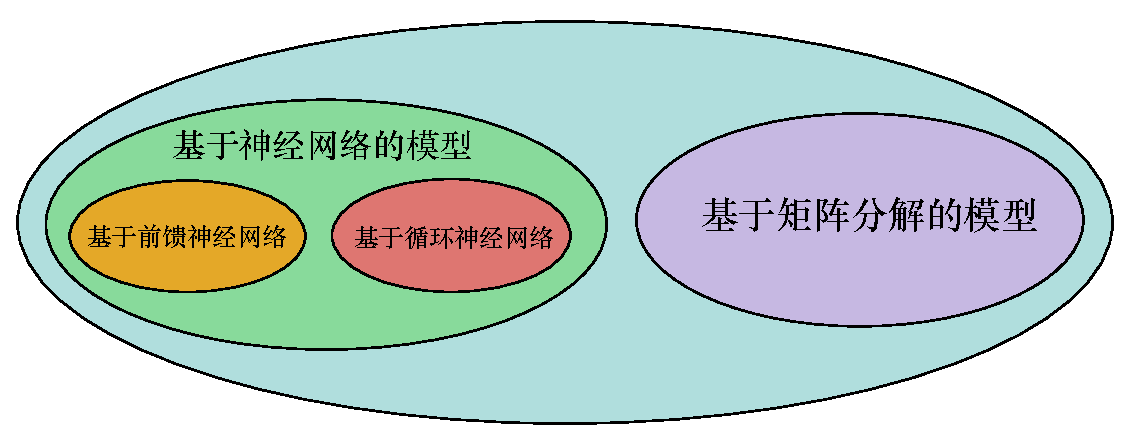
\includegraphics[width=\textwidth]{figures/train-venn.eps}
  \centering
  \caption{按照训练方法分类}
  \label{fig:train-venn}
\end{figure}

按照模型的训练方法来分,词向量模型可分为两大类:基于矩阵分解的模型和基于神经网络的模型,如 \cref{fig:train-venn} 所示。
基于神经网络的模型的共同特征是使用随机梯度下降和反向传播
\cite{Rumelhart:1988:LRB:65669.104451}进行参数的学习,具体又可分为使用前馈神经网络
(Feed Forward Neutral Network)和使用循环神经网络(Recurrent Neutral Network)的模型。

\subsubsection{基于矩阵分解的模型}
基于矩阵分解的模型以潜在语义分析(Latent Semantic Analysis,LSA)
\cite{DBLP:journals/jasis/DeerwesterDLFH90}和正定矩阵分解(Non-negative Matrix Factorization)为代表。
当词向量的维度较高或词汇表较大时,这些模型的训练非常耗时,所以在此不作过多的讨论。

\subsubsection{基于前馈神经网络的模型}

\paragraph{模型体系结构}
\begin{figure}
  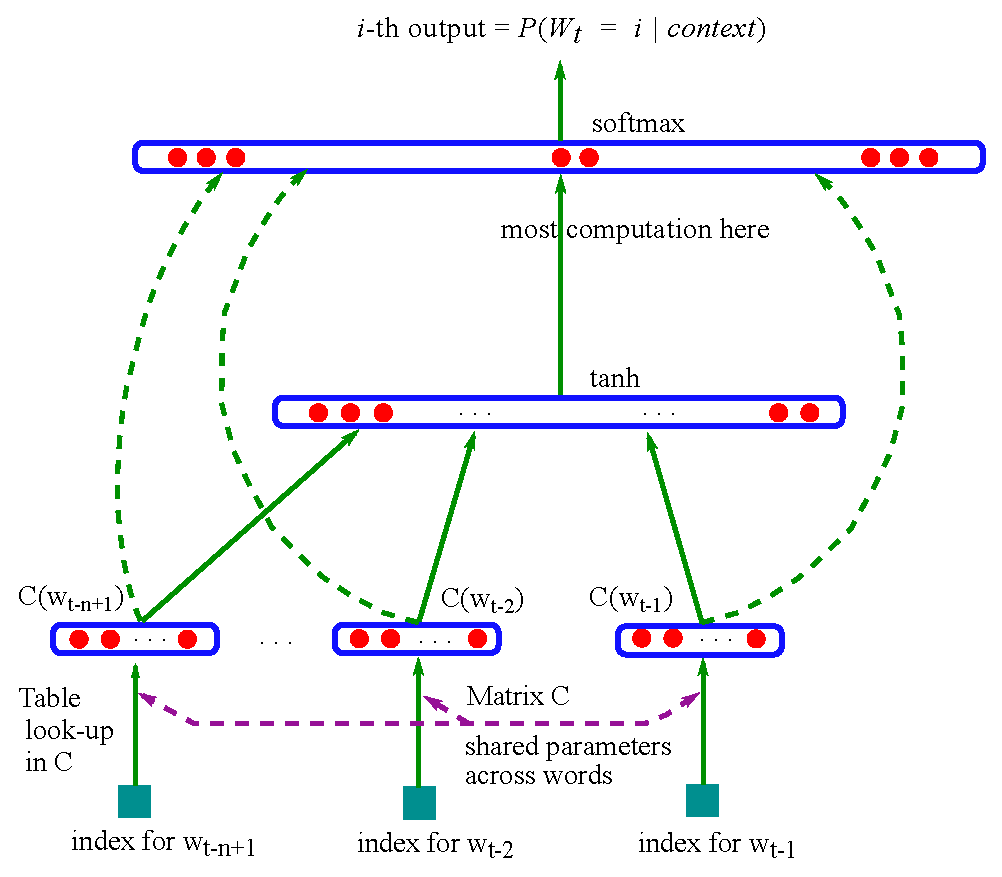
\includegraphics[width=0.8\textwidth]{figures/NNLM-arch.eps}
  \centering
  \caption{NNLM模型体系结构\cite{Bengio2006}}
  \label{fig:NNLM-arch}
\end{figure}

用于训练词向量的前馈神经网络由Bengio等人在\cite{DBLP:journals/jmlr/BengioDVJ03}中提出。
它包括了一个输入层、投影层、隐藏层和输出层。在输入层,$N$个历史词通过$1-V$独热编码($V$是词汇表的大小)。
随后,输入层被投影到一个维度为$N \times D$的投影层$P$($D$是词向量的维度)。
隐藏层使用神经网络中常见的激活函数($\tanh(x)$,$\sigma(x)$等)为模型引入非线性性。
输出层是维度为$V$的softmax,用于计算词在词汇表中的概率分布。词向量从模型的投影层获取。

\paragraph{计算复杂度}
NNLM的计算复杂度如下:
\begin{align}
  Q = N \times D + N \times D \times H + H \times V
  \label{eqn:nnlm-complexity}
\end{align}
其中决定性的是输出层的复杂度$H \times V$。然而,通过使用
分层softmax或者在训练时不对模型进行完全的正则化, 输出层的复杂度可以减至大约$\log_2(V)$。
因此,大部分的计算复杂度是在$N \times D \times H$项。

\paragraph{讨论}
优点:和n-gram模型相比,NNLM使用分布式的词表示,获得了更好的泛化。而且,NNLM在一个模型中同时获得了词向量和语言的概率模型。
局限性:模型使用了完整的神经网络,而隐藏层对习得词向量并非必要;模型对整个词汇表进行softmax,代价高昂。

\subsubsection{基于循环神经网络的模型}

\paragraph{模型体系结构}
\begin{figure}
  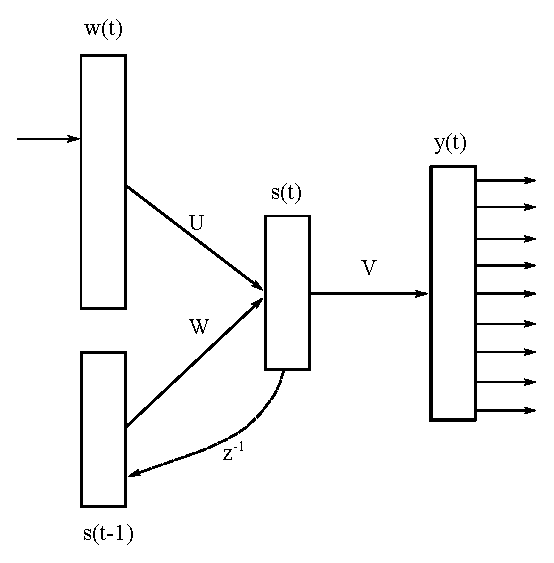
\includegraphics[width=0.6\textwidth]{figures/rnn-rvecs.eps}
  \centering
  \caption{循环神经网络模型体系结构\cite{DBLP:conf/interspeech/MikolovKBCK10}}
  \label{fig:rnn-arch}
\end{figure}

用于训练词向量的循环神经网络由Mikolov等人在\cite{DBLP:conf/interspeech/MikolovKBCK10}中提出。
模型由一个输入层,一个带有循环连接的隐藏层和输出层构成。
输入向量$\mathbf{w}(t)$表示独热编码的,在时刻$t$输入的词。
输出层$\mathbf{y}(t)$产生一个词的概率分布。
隐藏层$\mathbf{s}(t)$维护了一个句子历史的表示。
输入向量$\mathbf{w}(t)$和输出向量$\mathbf{y}(t)$的维度是词汇表的大小。
隐藏层和输出层的参数的计算如下:
\begin{align}
  \mathbf{s}(t) = f(\mathbf{Uw} & (t) + \mathbf{Ws}(t-1)) \\
  \mathbf{y}(t) = & g(\mathbf{Vs}(t))
  \label{eqn:rnn-arch}
\end{align}

其中:
\begin{align}
  f(z) = \frac{1}{1+e^{-z}}, \quad g(z_m) = \frac{e^{z_m}}{\sum_k e^{z_k}}
\end{align}
在此模型中,词向量为$\mathbf{U}$的行向量。

\paragraph{计算复杂度}
每一个训练样例的的复杂度是:
\begin{align}
  Q = H \times H + H \times V
  \label{eqn:rnn-complexity}
\end{align}
$H$是词向量的维度。
项$H \times V$可以通过分层softmax被有效的减至$H \times \log_2(V)$。
主要的复杂度来自$H \times H$。

\paragraph{讨论}
优点:不需要指定上下文的长度(模型的$N$参数); 可以有效的表达比浅层神经网络更复杂的模式
\cite{DBLP:conf/interspeech/MikolovKBCK10}
\cite{40d5d7fd62cb44ba934a8a75d4b2b076}。
局限性:带有有循环连接的隐藏层,计算开销高昂。
